\begin{enumerate}
	
	\item If A and B are two events such that 
		\begin{align}
			\pr{A|B} = 2 \times  \pr{B|A}\pr{A} + \pr{B}  = \frac{2}{3}
		\end{align}then \pr{B}  is equal to
\begin{enumerate}
\item $\frac{2}{9}$
\item $\frac{7}{9}$
\item $\frac{4}{9}$
\item $\frac{5}{9}$
\end{enumerate}

\item
\begin{enumerate}
\item Two balls are drawn at random one by one with replacement from an urn containing equal number of red balls and green balls. Find the probability distribution of number of red balls. Also, find the mean of the random variable.
\item A and B throw a die alternately till one of them gets '6' and wins the game. Find their respective probabilities of winning, if A starts the game first.
\end{enumerate}

\item Recent studies suggest that roughly $12\%$ of the world population is left handed.
	
\begin{figure}[h!]
\centering
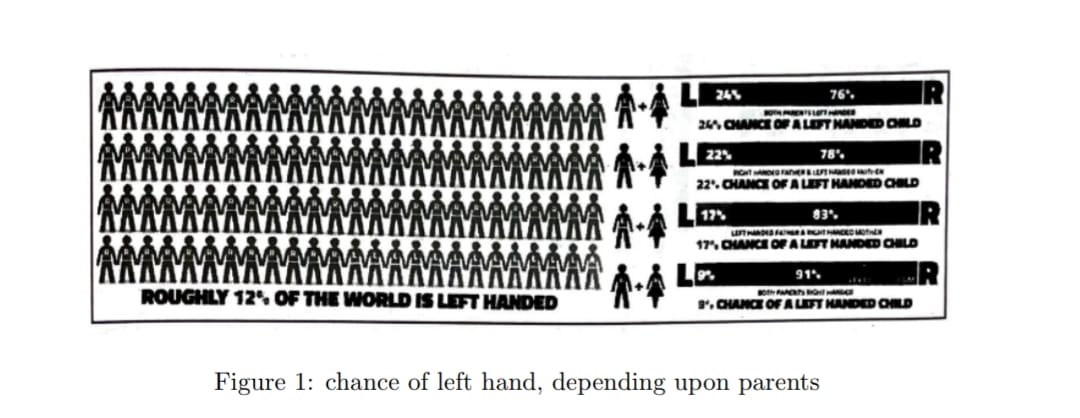
\includegraphics[width=\columnwidth]{figs/left.png}
\caption{chance of left hand, depending upon parents}
\label{fig:left.png}
\end{figure}

Depending upon the parents, the chances of having a left handed child are as follows :\\
\begin{enumerate}
\item   When both father and mother are left handed :
        Chances of left handed child is $24\%$.
\item   When father is right handed and mother is left handed :
        Chances of left handed child is $22\%$.
\item   when father is left handed and mother is right handed :
        Chances of left handed child is $17\%$.
\item   When both father nd mother are right handed :
        Chances of left handed child is $9\%$.
\end{enumerate}
Assuming that $\pr{A}=\pr{B}=\pr{C}=\pr{D}=\frac{1}{4}$ and L denotes the event that child is left handed.
Based on the above information, answer the following questions :\\
\begin{enumerate}
	\item    Find \pr{L|C}
	\item    Find \pr{\overline{L}|A}
	\item    Find \pr{A|L}
\item    Find the probability that a randomly selected child is left handed given that exactly one of the parent is left handed.
\end{enumerate}
\end{enumerate}
